\documentclass{beamer}
\usepackage{beamerthemesplit}
\usepackage{wrapfig}
\usetheme{SPbGU}
\usepackage{pdfpages}
\usepackage{amsmath}
\usepackage{cmap} 
\usepackage[T2A]{fontenc} 
\usepackage[utf8]{inputenc}
\usepackage[english,russian]{babel}
\usepackage{indentfirst}
\usepackage{amsmath}
\usepackage{tikz}
\usepackage{multirow}
\usepackage[noend]{algpseudocode}
\usepackage{algorithm}
\usepackage{algorithmicx}
\usetikzlibrary{shapes,arrows}
%usepackage{fancyvrb}
%\usepackage{minted}
%\usepackage{verbments}


\title[Теория формальных фзыков]{Формальные языки: практическое применение и теоретические вопросы}
\subtitle[]{Cеминар по алгоритмической математике \\ ЛЭТИ }
% То, что в квадратных скобках, отображается в левом нижнем углу. 
\institute[]{
Лаборатория языковых инструментов JetBrains \\
Санкт-Петербургский государственный университет \\
Математико-механический факультет }

% То, что в квадратных скобках, отображается в левом нижнем углу.
\author[Семён Григорьев]{Семён Григорьев}

\date{5 октября 2018г.}

\definecolor{orange}{RGB}{179,36,31}

\begin{document}
{
\begin{frame}[fragile]
  \begin{tabular}{p{2.5cm} p{5.5cm} p{2cm}}
   \begin{center}
      
\includegraphics[height=1.5cm]{pictures/JBLogo3.pdf}
    \end{center}
    &
    \begin{center}
      %
\includegraphics[height=1.5cm]{pictures/SPbGU_Logo.png}
    \end{center}
    &
    \begin{center}
      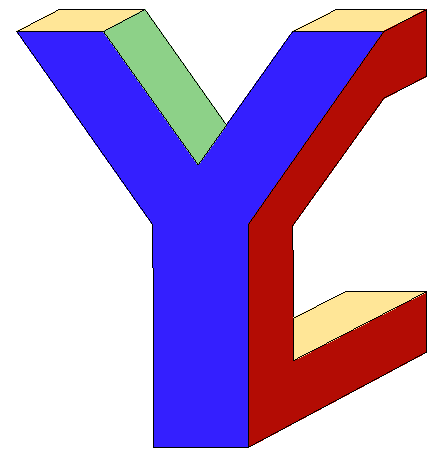
\includegraphics[height=1.5cm]{pictures/YC_logo.pdf}
    \end{center} 
  \end{tabular}
  \titlepage
\end{frame}
}

\begin{frame}[fragile]
  \transwipe[direction=90]
  \frametitle{Кто?}
  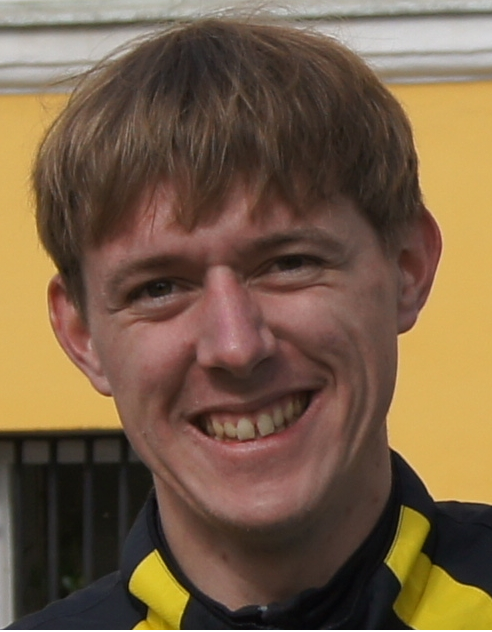
\includegraphics[height=2.5cm]{pictures/SemyonGrigorev.png}
  \\
  Семён Вячеславович Григорьев
  \begin{itemize}
    \item e-mail: \url{rsdpisuy@gmail.com}
    \item Исследователь в лаборатории языковых инструментов JetBrains Research
    \begin{itemize}
      \item \url{https://research.jetbrains.org/researchers/gsv}
    \end{itemize}
    \item к.ф.-м.н., доцент кафедры информатики СПбГУ
  \end{itemize}
\end{frame}

\begin{frame}[fragile]
  \transwipe[direction=90]
  \frametitle{Что?}
  Теория формальных языков
  \begin{itemize}
    \item Прикладные задачи
    \begin{itemize}
      \item Алгоритмы синтаксического анализа, восстановления после ошибок
      \item Статический анализ кода
      \item Алгоритмы выполнения запросов к граф-структурированым данным
    \end{itemize}
    \item Теоретические задачи
    \begin{itemize}
      \item Улучшение сложностных оценок алгоритмов
      \item ``Альтернативные'' взгляды на формальные языки
    \end{itemize}
  \end{itemize}
\end{frame}

\begin{frame}[fragile]
  \transwipe[direction=90]
  \frametitle{Где?}  
  \begin{itemize}
    \item GitHub-сообщество YaccConstructor: \url{https://github.com/YaccConstructor}
    \item Семинар по формальным языкам: \url{https://vk.com/ycformallanguagesseminar}
  \end{itemize}
\end{frame}


\begin{frame}[fragile]
\transwipe[direction=90]
\frametitle{О пересечении языков}
  \begin{itemize}
    \item Общая постановка вопроса
    \item Примеры постановок, имеющих прикладные значения
  \end{itemize}
  
\end{frame}

\begin{frame}[fragile]
\transwipe[direction=90]
\frametitle{Задачи}
                 
  \begin{itemize}
    \item Переход от произвольных контекстно-свободных ограничений к ограничениям в форме языка 
    Дика на двух типах скобок 
    \begin{itemize}
         \item GitHub:\url{https://github.com/YaccConstructor/YaccConstructor/issues/328}
    \end{itemize}

    \item Построение группы по языку
    \begin{itemize}
         \item Конспект: \url{https://v2.overleaf.com/19840442tgycbvgptdss}
         \item Больше материалов по группам и языкам: \url{https://github.com/YaccConstructor/YaccConstructor/issues/303}
    \end{itemize}

    \item Высокопроизводительный алгоритм поиска путей с контекстно-свободными ограничениями
    \begin{itemize}
         \item На CPU. GitHub:\url{https://github.com/YaccConstructor/YaccConstructor/issues/320}
         \item На GPGPU. GitHub:\url{https://github.com/YaccConstructor/YaccConstructor/issues/321}
    \end{itemize}

  \end{itemize}
  
\end{frame}


\begin{frame}[fragile]
\transwipe[direction=90]
\frametitle{Больше задач}
                 
  \begin{itemize}
    \item Поиск путей с ограничениями в виде конъюнктивных грамматик
    \begin{itemize}
         \item GitHub:\url{https://github.com/YaccConstructor/YaccConstructor/issues/311}
    \end{itemize}

    \item Производные (Brzozowski’s derivatives) для поиска путей с КС ограничениями
    \begin{itemize}
         \item GitHub: \url{https://github.com/YaccConstructor/YaccConstructor/issues/306}
    \end{itemize}

    \item Можно поизучать issues в репозиториях сообщества.
    \begin{itemize}
         \item Там даже есть метки для фильтрации
         \item но они условны
    \end{itemize}

  \end{itemize}
  
\end{frame}


\end{document}
